\subsection{Comparison with a dissipative network}
\label{sec:res_compare}

A virtual spring--damper network~\cite{quan2025swarm} is the natural comparison for a team that changes in flight: a
member leaving or joining needs no new solver. We ported Quan et al.'s dissipative network to our system and flew it
against our planner in the twin. Four carriers sit on plates 0, 3, 6 and 9, with 1\,m cables and the ring at 1.0\,m.
The cases are a hover and a 0.9\,m line out and back. Both arms are our planner up to the hand-over (creep, lift and a
5\,s hover). After it, our arm keeps the planner of Sec.~\ref{sec:method} and its trackers. The network instead drives
the trackers' velocity loop with no integral per UAV. The comparison is therefore between the two methods as flown
after the lift, not of the network alone. The port follows the authors' simulation code (a network of integrated virtual nodes) rather
than the per-robot law of the paper's text, and it turns the formation with the ring's measured attitude, because
our ring has an attitude and the paper's payload does not. Every run is exploratory, one or two per cell
(Table~\ref{tab:compare}).

\emph{As ported, the network capsizes in yaw.} At its first gains the ring's yaw swung with a growing amplitude, in
hover and on the line at 0.2\,m/s, until the ring tipped past the abort limit (Fig.~\ref{fig:c_yaw}). A bounded
offline retune followed, set before the comparison flew: a grid over the damping and the velocity loop's position gain,
then a descent over eight gains, ranked on safety guards and then on the line's error at 0.4\,m/s. At the search's best
gains the network held the ring through every scored window, but not its yaw (in one hover run the ring tipped past
30$^\circ$ 64\,s after the hand-over, 4\,s after the window, before the landing): the yaw swung through 22--51$^\circ$ in hover and about
14$^\circ$ on the 0.4\,m/s line. On that line its error was 99--105\,mm against our planner's 44--46\,mm, about twice as
large. The network also ran about 1.1\,s behind the schedule and turned short of each end (Fig.~\ref{fig:c_line}).
Our planner ran 0.03\,s late and its ring's yaw moved 0.2$^\circ$. In every case each run of our planner was closer
than each run of the retuned network: 1.3--1.4 against 16.1--18.7\,mm in hover and 17.0--17.6 against 41.5--42.1\,mm
on the 0.2\,m/s line.

\emph{Why the yaw is lost.} The paper models the load as a point, with every cable attached at its centre of
mass~\cite{quan2025swarm}. Our ring hangs from plates on its rim, at 0.225\,m from the axis. The cables then torque the
ring, which gives it a yaw mode that the method has no term for, and the attitude-following formation of our port
feeds that mode. To test this we moved every cable's lower end to a hub at the ring's centre, which is the paper's own
geometry, and changed nothing else. With two runs per case, the network at its best gains held the ring's yaw within 0.1$^\circ$ in hover and
0.2$^\circ$ on the 0.2\,m/s line, against 22--51$^\circ$ and 29--48$^\circ$ on the rim; on the 0.4\,m/s line it
still swung through 20--28$^\circ$. Its hover error fell by 30\,\% (17.4 to 12.2\,mm on average), but its line errors
did not move (40 against 42\,mm and 102 against 102\,mm). On the hub, too, each run of our planner was closer than each
run of the network, though on the lines our planner did worse than on the rim, for a reason not yet tested. The
network exactly as ported, which lost the ring on the rim, held it on the hub in its single run per case. The paper's
own form of the damping and feed-forward, at the gains that were best offline, lost the ring on the rim in all six
runs: it tipped past 30$^\circ$ 20--30\,s after the hand-over.

The result is about porting a point-load method to a rigid ring hung from its rim, not a verdict on Quan et al.'s
method as published. Its formation, its damping and its decentralised structure are untouched by it. What the rim
attachment adds is a rotational state that a team carrying a rigid ring must regulate; our planner held it on both
geometries.

\begin{table}[t]
\centering
\footnotesize
\setlength{\tabcolsep}{4pt}
\caption{Our planner against our port of the dissipative network~\cite{quan2025swarm} in the twin, four carriers on
1\,m cables, rim plates unless marked hub; 1--2 runs per cell. Error: in hover the ring's 3-D error; on a
line the clock-free error plus the shortfall at the line's ends. Lag: behind the schedule. Yaw: the ring's largest
change of yaw after the hand-over. $^a$Lost the ring (tilt past 30$^\circ$); the run aborted and its error is not
scored. Hub cells: two runs each, one code tree.}
\label{tab:compare}
\begin{tabular}{@{}llccc@{}}
\toprule
Arm & Case & Error (mm) & Lag (s) & Yaw ($^\circ$) \\
\midrule
Our planner & hover & 1.3--1.4 & -- & 0.0--0.1 \\
 & line 0.2\,m/s & 17.0--17.6 & $+$0.09--0.10 & 0.1 \\
 & line 0.4\,m/s & 44.3--46.2 & $+$0.03 & 0.2 \\
\addlinespace
Network, as ported & hover & --$^a$ & -- & 125 \\
 & line 0.2\,m/s & --$^a$ & -- & 474 \\
\addlinespace
Network, retuned & hover & 16.1--18.7 & -- & 22--51 \\
 & line 0.2\,m/s & 41.5--42.1 & $+$1.25 & 29--48 \\
 & line 0.4\,m/s & 99.3--104.5 & $+$1.12--1.13 & 14 \\
\addlinespace
Network, paper's form & all three & --$^a$ & -- & -- \\
\addlinespace
Our planner, hub & hover & 1.4 & -- & 0.0 \\
 & line 0.2\,m/s & 30.0--32.2 & $+$0.16--0.18 & 0.2 \\
 & line 0.4\,m/s & 71.1--73.9 & $+$0.05--0.06 & 0.1--0.2 \\
\addlinespace
Network, retuned, hub & hover & 11.8--12.5 & -- & 0.1 \\
 & line 0.2\,m/s & 40.0--40.1 & $+$1.25 & 0.2 \\
 & line 0.4\,m/s & 101.6--103.3 & $+$1.14--1.15 & 20--28 \\
\bottomrule
\end{tabular}
\end{table}

\begin{figure}[t]
\centering
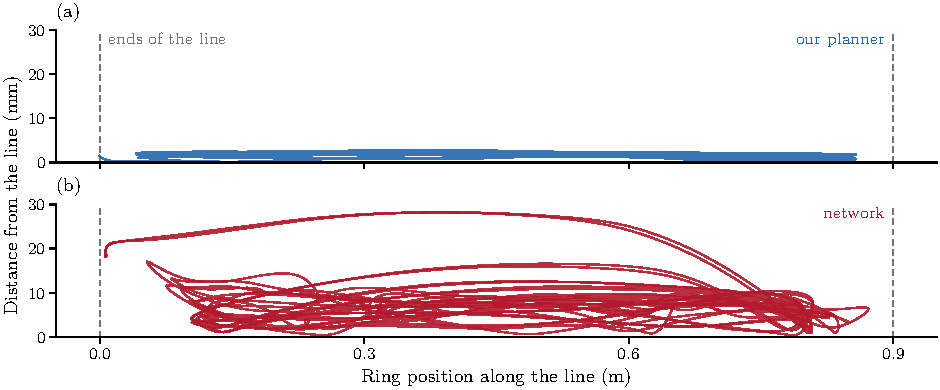
\includegraphics[width=\columnwidth]{figures/fig_c_line.pdf}
\caption{The 0.4\,m/s line in the twin: the ring's position along the line against the schedule, our planner and the
retuned network. The network runs about 1.1\,s late and turns short of each end.}
\label{fig:c_line}
\end{figure}

\begin{figure}[t]
\centering
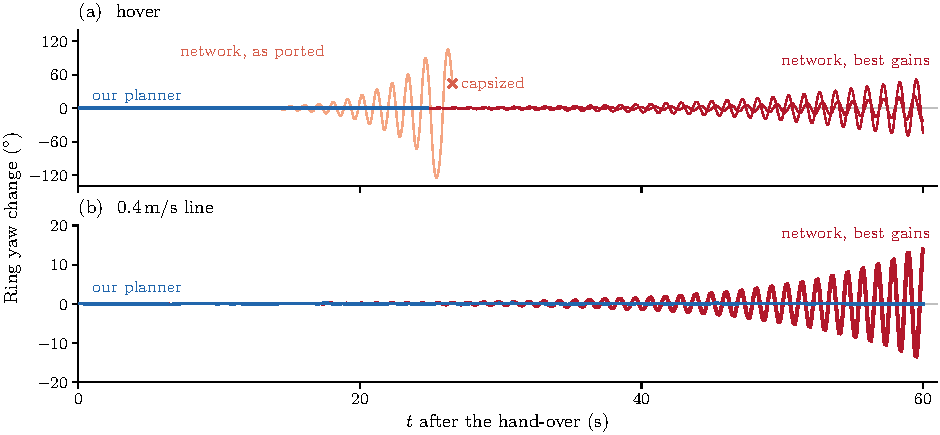
\includegraphics[width=\columnwidth]{figures/fig_c_yaw.pdf}
\caption{The ring's yaw after the hand-over in hover: the network as ported (it capsizes and the run aborts), the
retuned network (the yaw swings but the ring is held), and our planner.}
\label{fig:c_yaw}
\end{figure}
